\documentclass[xcolor=x11names,compress,professionalfonts, aspectratio=169]{beamer}

%% General packages %%%%%%%%%%%%%%%%%%%%%%%%%%%%%%%%%%
\usepackage[utf8]{inputenc}
\usepackage{graphicx}
\usepackage{tikz}
\tikzset{% change default arrow tips
    >=latex
}
\usepackage{ifthen}

\usepackage{amsmath}
\usepackage{nicefrac}

\usepackage{color}

% compile child documents using this preamble
\usepackage{subfiles}

% compile child files with separate preambles, and include them in the document
\usepackage{standalone}

%%%%%%%%%%%%%%%%%%%%%%%%%%%%%%%%%%%%%%%%%%%%%%%%%%%%%%

\makeatletter
\setbeamertemplate{footline}
{
    \leavevmode%
    \hbox{%
        \begin{beamercolorbox}[wd=.333333\paperwidth,ht=2.25ex,dp=1ex,center]{author in head/foot}%
            \usebeamerfont{author in head/foot}\insertshortauthor
        \end{beamercolorbox}%
                \begin{beamercolorbox}[wd=.333333\paperwidth,ht=2.25ex,dp=1ex,center]{title in head/foot}%
            \usebeamerfont{title in head/foot}\insertshorttitle
        \end{beamercolorbox}%
        \begin{beamercolorbox}[wd=.333333\paperwidth,ht=2.25ex,dp=1ex,right]{date in head/foot}%
            \usebeamerfont{date in head/foot}\insertshortdate{}\hspace*{2em}
            \insertframenumber{} / \inserttotalframenumber\hspace*{2ex} 
        \end{beamercolorbox}}%
        \vskip0pt%
    }
    \makeatother


%% Beamer Layout %%%%%%%%%%%%%%%%%%%%%%%%%%%%%%%%%%
\useoutertheme[subsection=false,shadow]{miniframes}
\useinnertheme{rectangles}

\setbeamertemplate{navigation symbols}{}%remove navigation symbols

\author{Nicolas Macé}

\newcommand{\btVFill}{\vskip0pt plus 1filll}%place an element at the bottom of the page

\usepackage{libertine}
\usepackage[T1]{fontenc}

\setbeamerfont{title like}{shape=\scshape}
\setbeamerfont{frametitle}{shape=\scshape}

\setbeamercolor*{lower separation line head}{bg=DeepSkyBlue4} 
\setbeamercolor*{normal text}{fg=black,bg=white} 
\setbeamercolor*{alerted text}{fg=red} 
\setbeamercolor*{example text}{fg=black} 
\setbeamercolor*{structure}{fg=black} 
 
\setbeamercolor*{palette tertiary}{fg=black,bg=black!10} 
\setbeamercolor*{palette quaternary}{fg=black,bg=black!10} 

\renewcommand{\(}{\begin{columns}}
\renewcommand{\)}{\end{columns}}
\newcommand{\<}[1]{\begin{column}{#1}}
\renewcommand{\>}{\end{column}}

\definecolor{BostonBlue}{HTML}{00688B}
\definecolor{Complementary}{HTML}{8B2300}

% letters A and B appearing in the qp chains
\newcommand{\A}{\textcolor{BostonBlue}{A}}
\newcommand{\B}{\textcolor{Complementary}{B}}

\renewcommand{\ss}[1]{\scriptsize{\text{#1}}}
%%%%%%%%%%%%%%%%%%%%%%%%%%%%%%%%%%%%%%%%%%%%%%%%%%

\usepackage{braket}
% compile child documents using this preamble
\usepackage{subfiles}

%%%My Math

\newcommand{\pd}[2]{\frac{\displaystyle \partial #1}{\displaystyle\partial #2}} % for partial derivatives
\renewcommand{\d}[1]{\mathrm{d}#1}

\begin{document}

\begin{frame}
\title{{\fontsize{14}{60}\selectfont Exact results on electronic wavefunctions of 2D quasicrystals}}

\author{Nicolas Macé, Anuradha Jagannathan, Frédéric Piéchon}

\institute % (optional)
{
  Laboratoire de Physique des Solides\\
  Université Paris-Saclay
}

\date{November 23, 2016}

\titlepage

\btVFill
\begin{columns}
\begin{column}{2cm}
~\\
~\\
~\\
~\\
\raggedright

\includegraphics[scale=.15]{img/LogoUPSUD.png}
\end{column}
\begin{column}{6cm}
\centering
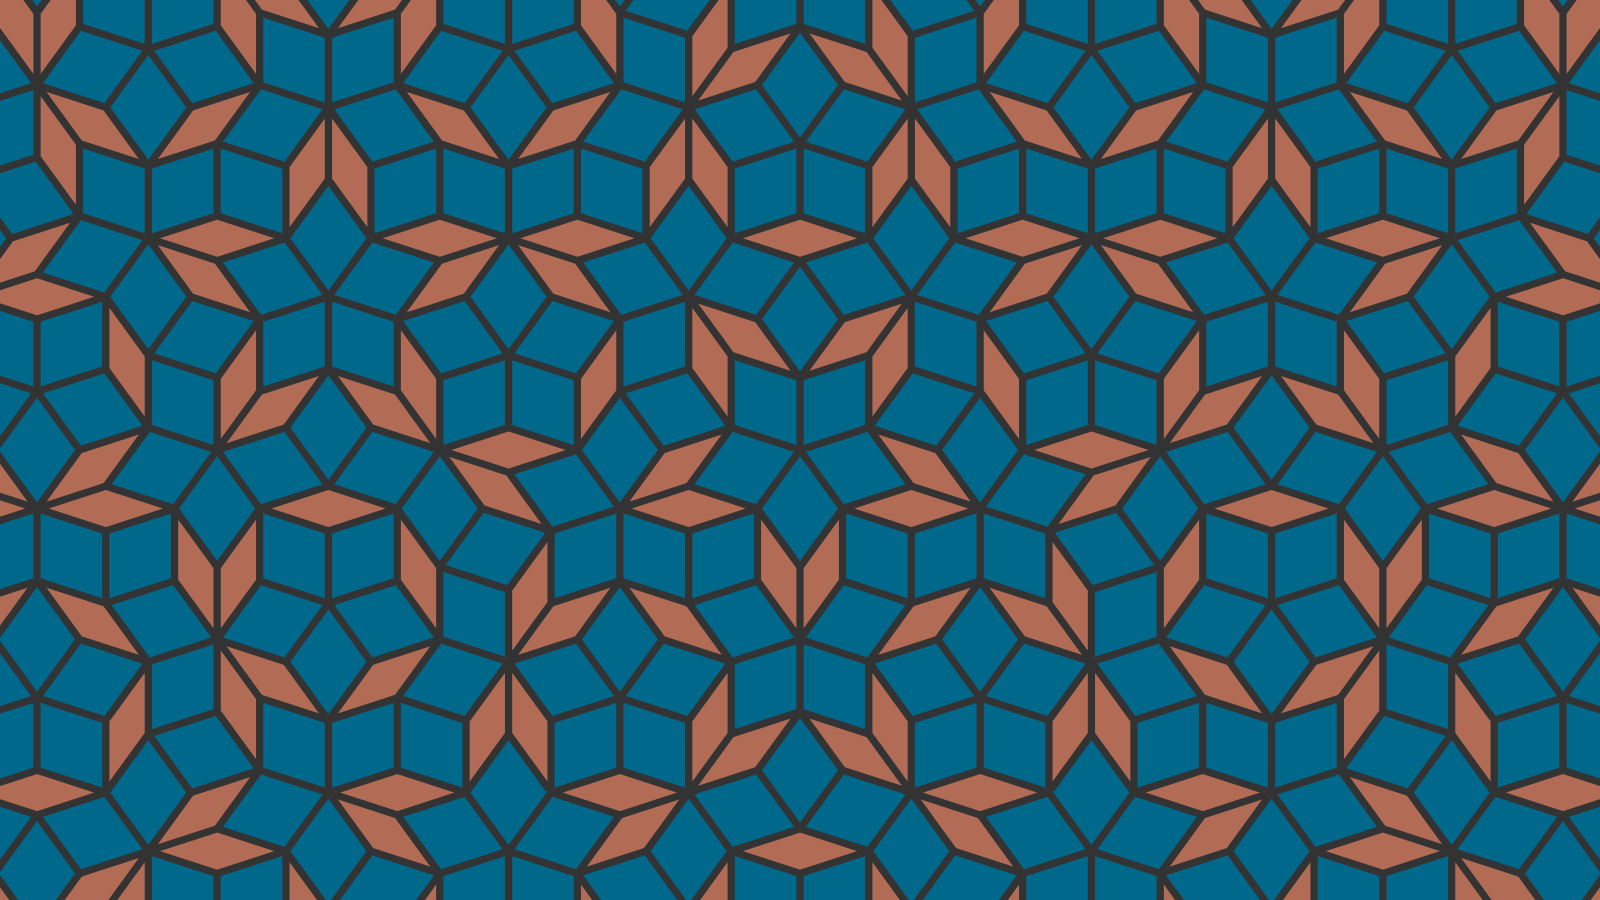
\includegraphics[width=.8\textwidth]{img/cover.png}
\end{column}
\begin{column}{2cm}
~\\
~\\
~\\
~\\
\raggedleft

\includegraphics[scale=.15]{img/logo-lps.jpg}
\end{column}
\end{columns}
\end{frame}

\begin{frame}{Electrons on quasicrystals}
\begin{itemize}
	\item In 1D (quasiperiodic chains): electronic spectrum and wavefunctions are well known. 
	\item In 2D and 3D: many numerical investigations, but almost no exact results.
\end{itemize}
$\rightarrow$ recent (big!) improvement: Kalugin, Katz (2014) guessed the groundstate of a large class of 2D models.

\begin{itemize}
	\item What does this groundstate look like?
	\item Which new insights does it bring us?
\end{itemize} 
\end{frame}

\begin{frame}
\frametitle{Toy models of quasicrystals}
We want to model:
\begin{itemize}
	\item a single electron (ie we do not consider interactions)
	\item on a quasiperiodic tiling, in 1D or in 2D
	\item in the simplest possible way : tight-binding model with nearest neighbors hoppings only
\end{itemize}

\begin{columns}
\<{5cm}
\[
	i \frac{\partial \phi_m}{\partial t}(t) = \sum_{n ~\text{NN}~m} t_{m,n} \phi_n(t)
\]
$|\phi_m(t)|^2= $ proba to be on atom $m$ at time $t$.
\>

\<{5cm}
\centering
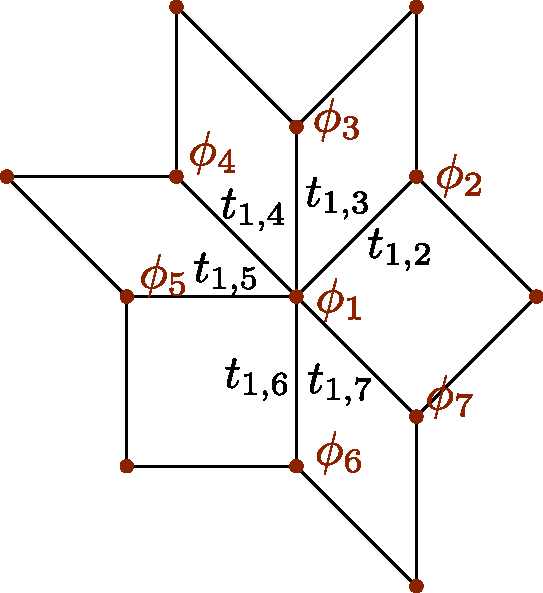
\includegraphics[scale=0.45]{img/ham_example.pdf}
\>

\<{5cm}
Solve for the stationary states (or eigenstates):
\[
	E \psi_m = \sum_{n ~\text{NN}~m} t_{m,n} \psi_n
\]
\>
\end{columns}
\end{frame}

\begin{frame}
\frametitle{Outline}
\tableofcontents[hideallsubsections]
\end{frame}

\begin{frame}
\frametitle{Periodic and disordered models}
\begin{itemize}
	\item Eigenstates on periodic materials: 
	\begin{itemize}
		\item Plane waves 
		\item \textbf{uniform} probability $\rightarrow$ \textbf{extended states}
	\end{itemize}
	\subfile{img/periodic_chain.tex}
	\item Eigenstates on disordered materials: 
	\begin{itemize}
		\item Evanescent waves
		\item  \textbf{exponentially decreasing} probability $\rightarrow$ \textbf{localized states}
	\end{itemize}
	\subfile{img/disordered_chain.tex}
\end{itemize}
\textbf{What about quasiperiodic materials?}

\textcolor{Complementary}{We will see on examples their electrons are somewhat \textbf{in between}: the wavefunctions have power law decays, they are \textbf{critical}}
\end{frame}

\section{1D model (Fibonacci chain): a ``baby example''}
%Each section needs a subsection for the small points on top to show up
\subsection{Dummy}

\begin{frame}{The Fibonacci chain}
		The geometrical model: a chain of two letters generated by the substitution
	\[	
	M: \left\{\begin{array}{ll} \A \to & \A \B \\ \B \to & \A
	\end{array}\right.	
	\]
		
{\centering
$M^{\infty}(\A) = \dots\A\B\A\B\A\A\B\A\A\B\A\B\A\A\B\A\B\A\dots $

}
		
		The corresponding chain of atoms:
		
		{\centering
		\subfile{img/fibo_chain.tex}
		
		}
The Schrödinger equation for the eigenstate of energy $E$:
\[
	 t_{m-1,m} \psi_{m-1} + t_{m,m+1}\psi_{m+1} = E \psi_{m}
\]
\[
	t_{m-1,m} = t_s \text{~or~} t_w \text{~we introduce the ratio $\rho = t_w / t_s$}
\]
What can be say about the spectrum/eigenstates of this model?
\end{frame}

\begin{frame}{Spectrum and eigenstates}
\begin{itemize}
	\item The spectrum is scale invariant (or multifractal)
	
{\centering
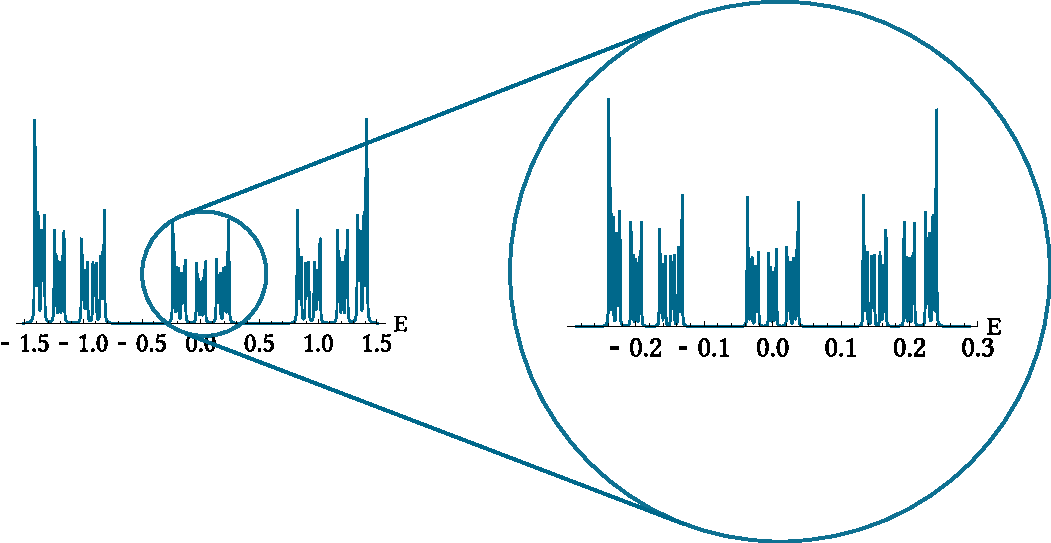
\includegraphics[scale=.5]{img/ldos.pdf}

\small{(Spectrum computed for $\rho=0.5$)}
}
	\item The eigenstates are all critical (neither localized nor extended)
\end{itemize}
What is the structure of these critical states?
\end{frame}

\begin{frame}{A baby example: the eigenstate at zero energy}
\begin{itemize}
	\item Schrödinger equation for the $E=0$ state:
	\[
	t_{m-1,m} \psi_{m-1} + t_{m,m+1}\psi_{m+1} = 0
	\]
	\item If we know the wavefunction on one site we know it on the next
	\begin{columns}
	\<{6cm}
	\[
	\psi_{m+1} = -\frac{t_{m-1,m}}{t_{m,m+1}} \psi_{m-1}
	\]
	\>
	\<{5cm}
	\subfile{img/hop_E0.tex}
	\>
	\end{columns}
	\only<1>{
	\item There are 4 possible cases:
	
	\centering
	 \subfile{img/hop_1.tex}
	 }
	\only<2>{
	\item Introduce $A_{m-1,m+1}$, the \textbf{arrow} from $m-1$ to $m+1$:
	\begin{columns}
	\<{5cm}
	\centering
	 \subfile{img/hop_2.tex}
	 \>
	 \<{5cm}
	Then, $\boxed{\psi_{m+1} = \rho^{A_{m-1,m+1}} \psi_{m-1}}$
	 \>
	 \end{columns}
	 }
\end{itemize}
\end{frame}

\begin{frame}{The field of arrows and the field of heights}
Iterating $\psi_{m+1} = \rho^{A_{m-1,m+1}} \psi_{m-1}$,
\[
	\psi_{m} = \psi_0 \rho^{h(m)}
\]
Where $h$ is \textbf{the field of heights}, the integral of the field of arrows:
\[
	h(m) = \sum_{n=1}^{m/2} A_{2n-2, 2n}
\]

Example (piece of the Fibonacci chain):
\subfile{img/field_of_heights.tex}


\end{frame}

\begin{frame}{Back to the special cases, with arrows!}
\begin{itemize}
	\item Periodic chain: 
	\subfile{img/periodic_chain_arrows.tex}
	\begin{itemize}
		\item Arrows $= 0 \implies h(m) = 0 \implies \psi_m = \psi_0 \rho^{0} = $ cst  
		\item \textbf{uniform} probability $\rightarrow$ \textbf{extended states}
	\end{itemize}
	\item Disordered chain: 
	\subfile{img/disordered_chain_arrows.tex}
	\begin{itemize}
		\item Arrows randomly distributed $\implies h(m) \sim \langle A \rangle \times m \implies \psi_m \sim \rho^{\langle A \rangle \times m} \sim e^{- m/\xi}$ with $\xi^{-1} = |\log \rho| \langle A \rangle$
		\item  \textbf{exponentially decreasing} amplitude $\rightarrow$ \textbf{localized states}
	\end{itemize}
\end{itemize}
$\rightarrow$ expected behavior in both cases.

What happens for a quasiperiodic chain?
\end{frame}

\begin{frame}{The $E=0$ state is not localized}
\begin{columns}
\<{6cm}
Apply the substitution three times:
	\[	
	M^3: \left\{\begin{array}{ll} \A \to & \A \B \A \B \A \\ \B \to & \A \B \A
	\end{array}\right.	
	\]
\>
\<{6cm}
{
\centering
\subfile{img/atomic_inflation_no_localization.tex}
}
\>
\end{columns}
$\rightarrow$ the height is invariant under the substitution $M^3$: it doesn't change on the preexisting sites
\begin{itemize}
	\item the wavefunction doesn't change on the preexisting sites
	\item these preexisting sites get arbitrarily far apart as we iterate the substitution 
\end{itemize}
$\rightarrow$ we can find the electron with high probability arbitrarily far from the origin: \textbf{the wavefunction is not localized.}
\end{frame}

\begin{frame}{The $E=0$ state is not extended}
{

\centering
\subfile{img/atomic_inflation_no_extension.tex}
}

\begin{columns}
\<{7cm}
{\centering
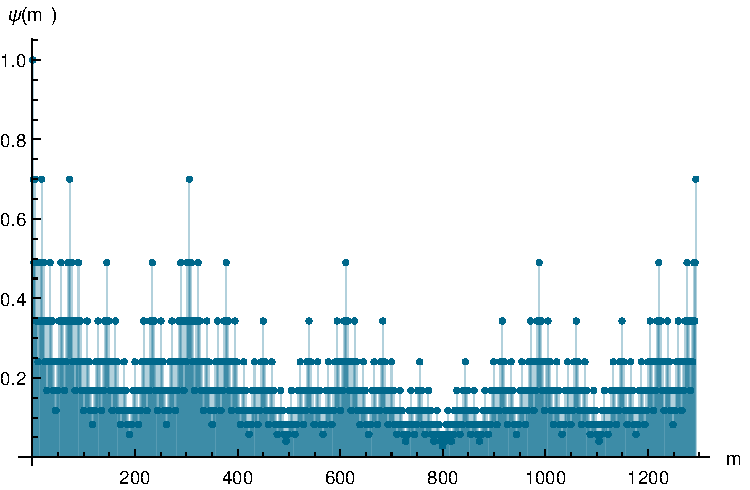
\includegraphics[scale=.5]{img/wavefunction.pdf}

}
\>

\<{7cm}
Local scale invariance:
\[
	\psi_{a \times m} = b \times \psi_{m} 
\]
$\rightarrow$ local \textbf{power law decay}
\[
\psi_{r_n} \sim r_n^\alpha, ~(\alpha = \log b/\log a)
\]
$\rightarrow$ \textbf{wavefunction is not extended}
\>
\end{columns}

\end{frame}

\begin{frame}{Cut and project chains: a summary}
\begin{itemize}
	\item The $E=0$ wavefunction of cut and project chains is described by a \textbf{height field}
	\item The height field is the integral of an \textbf{arrow field}, which is quasiperiodic
	\item Geometry of the tiling $\implies$ structure of the wavefunction
	\item $\rightarrow$ \textbf{the wavefunction is critical}: neither localized nor extended, behaves locally as a power law
\end{itemize}
We will find again all these features in 2D!
\end{frame}

\section{2D models (Penrose and Ammann-Beenker tilings): the ``grown-up example''}
\subsection{Dummy}

\begin{frame}{2D tilings}
We consider the Penrose and the Ammann-Beenker tilings.
\begin{columns}
\begin{column}{5cm}
{\centering
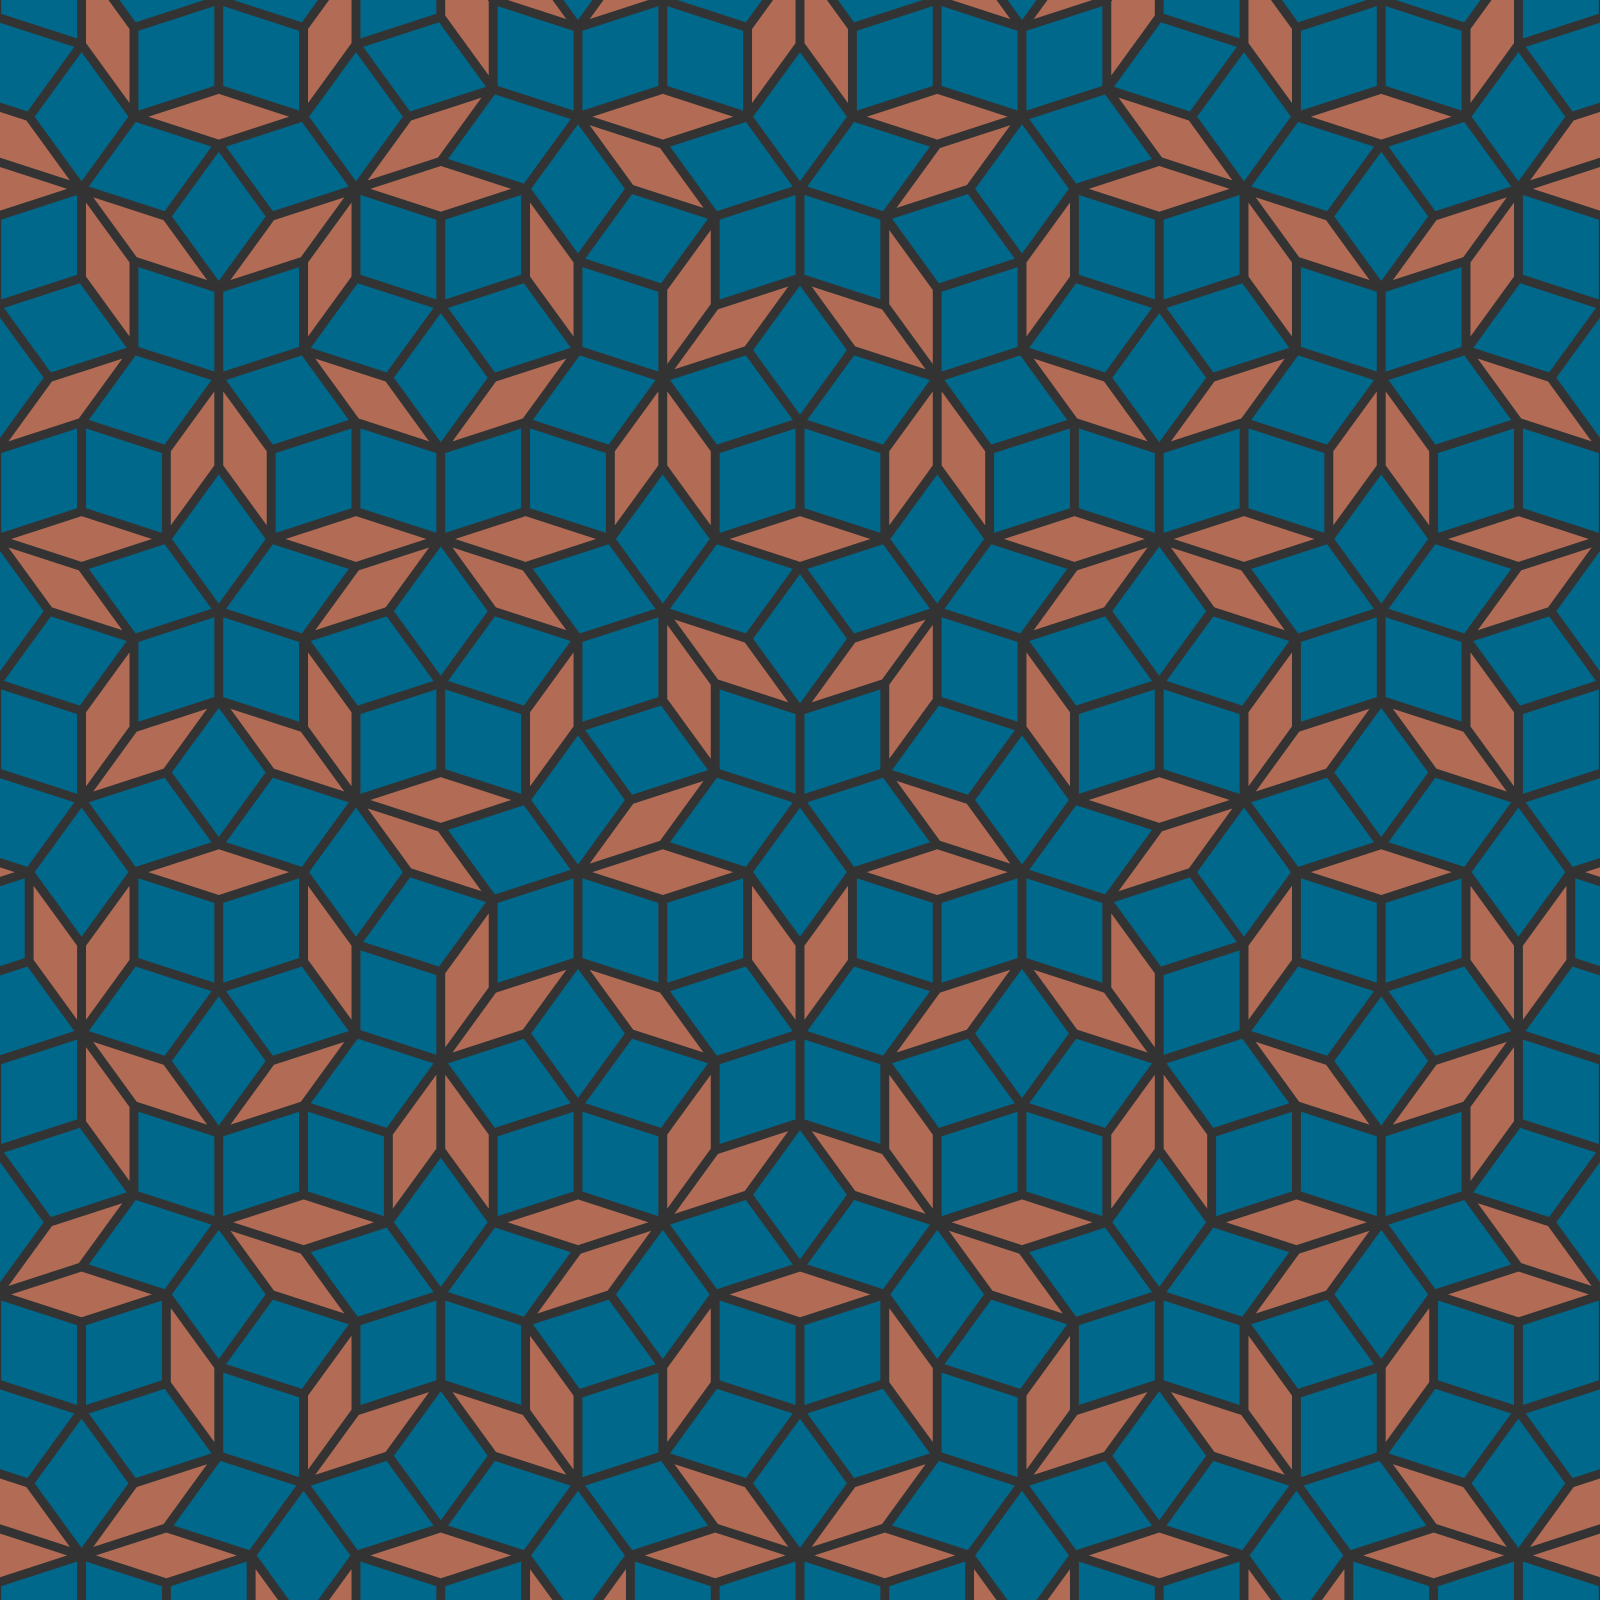
\includegraphics[scale=.09]{img/penrose.png}

}
\end{column}
\begin{column}{5cm}
{\centering
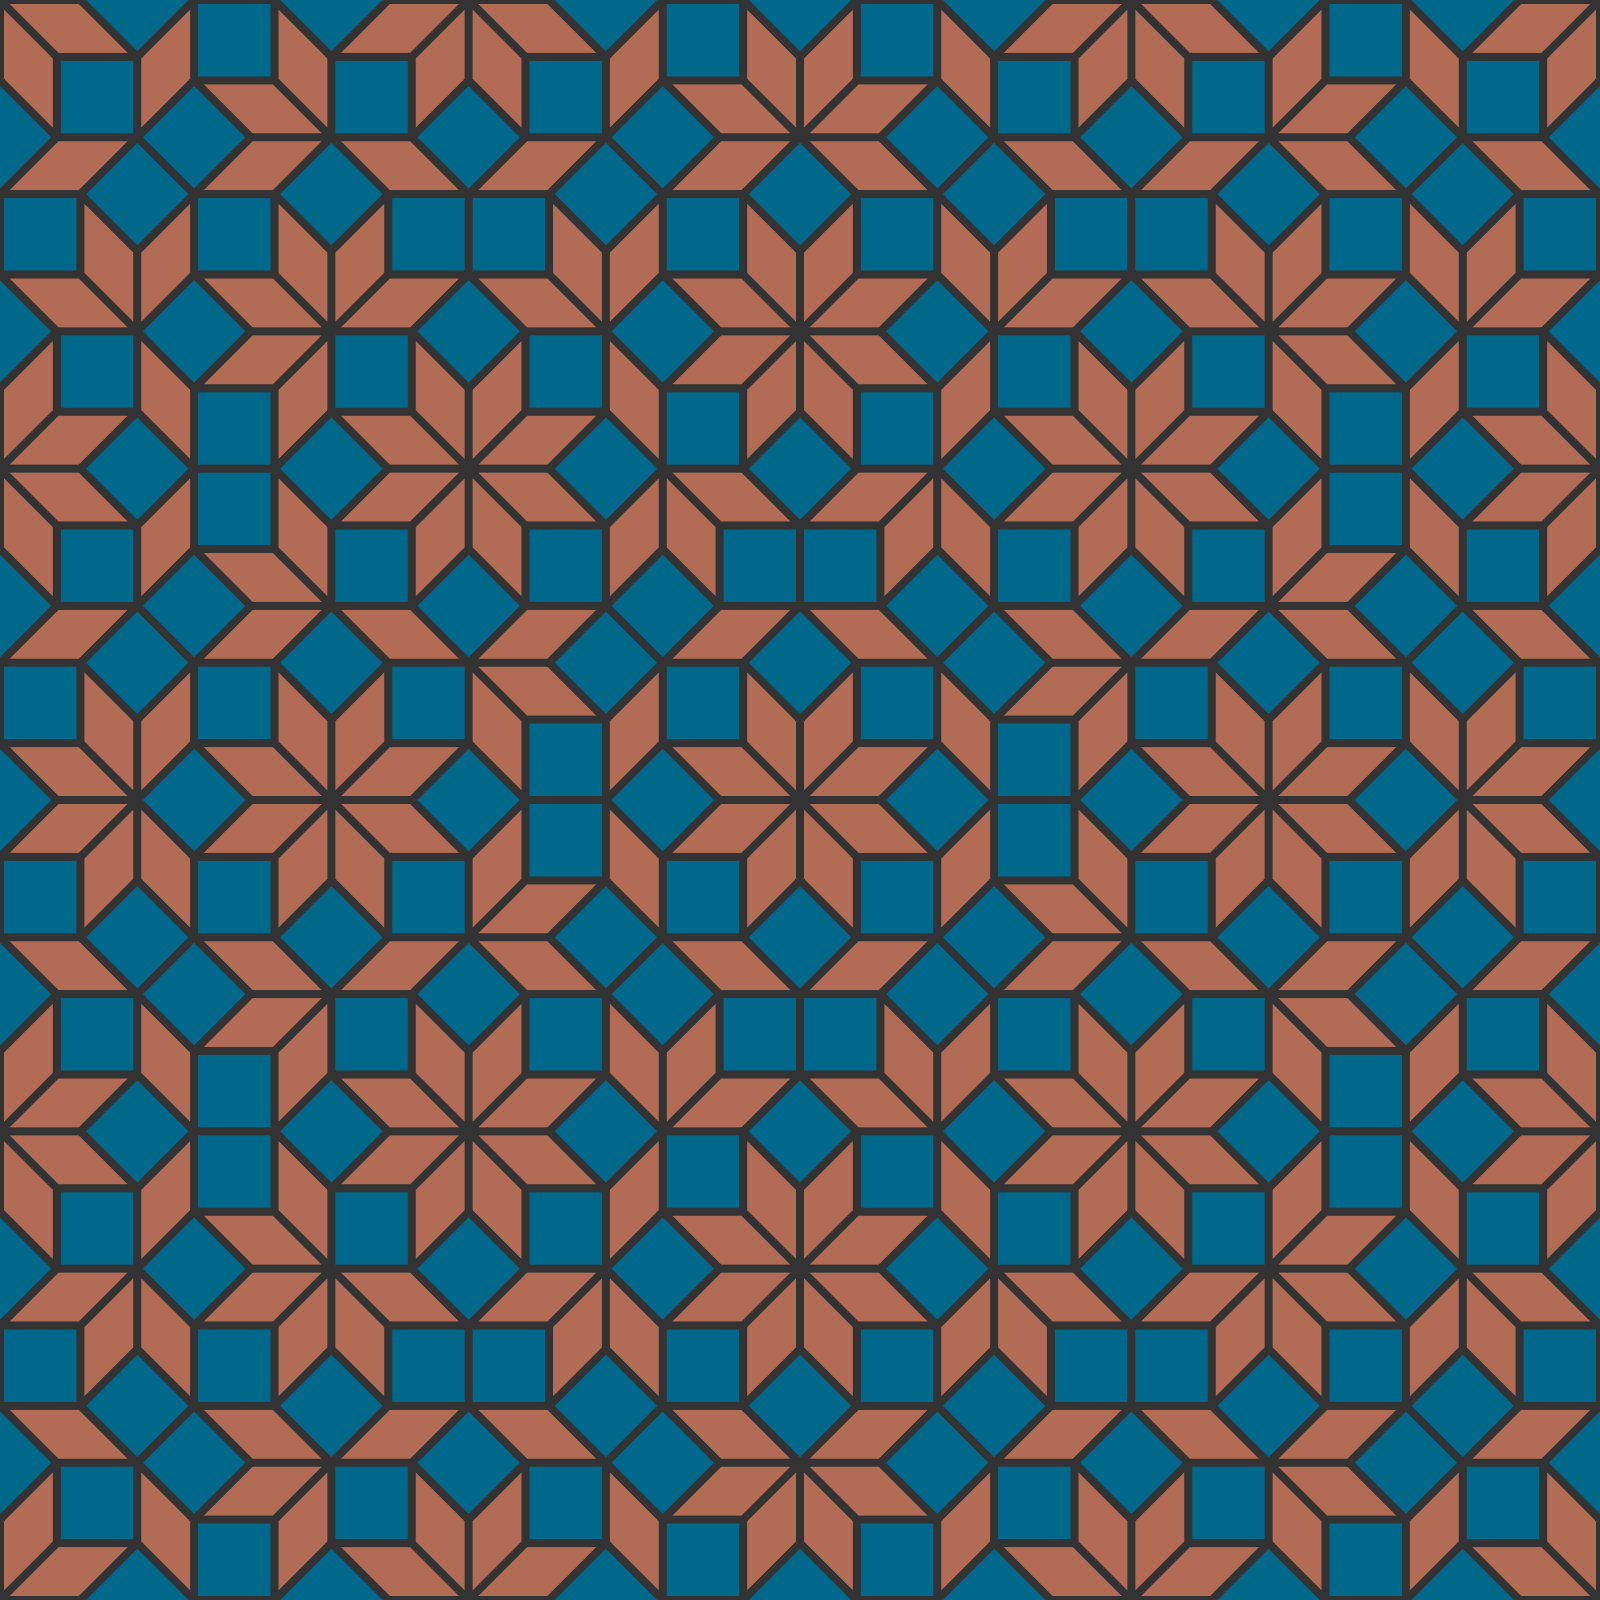
\includegraphics[scale=.09]{img/ammann-beenker.png}

}
\end{column}
\<{4cm}
Model for the electron:
\[
	E \psi_m = V_m \psi_m + \sum_{n ~\text{NN}~m} t \psi_n
\]

Quasiperiodicity encoded in the adjacency of the vertices
\>
\end{columns}

\end{frame}

\begin{frame}{What is known}

Local density of states [taken from Zijlstra 2014]:

{\centering
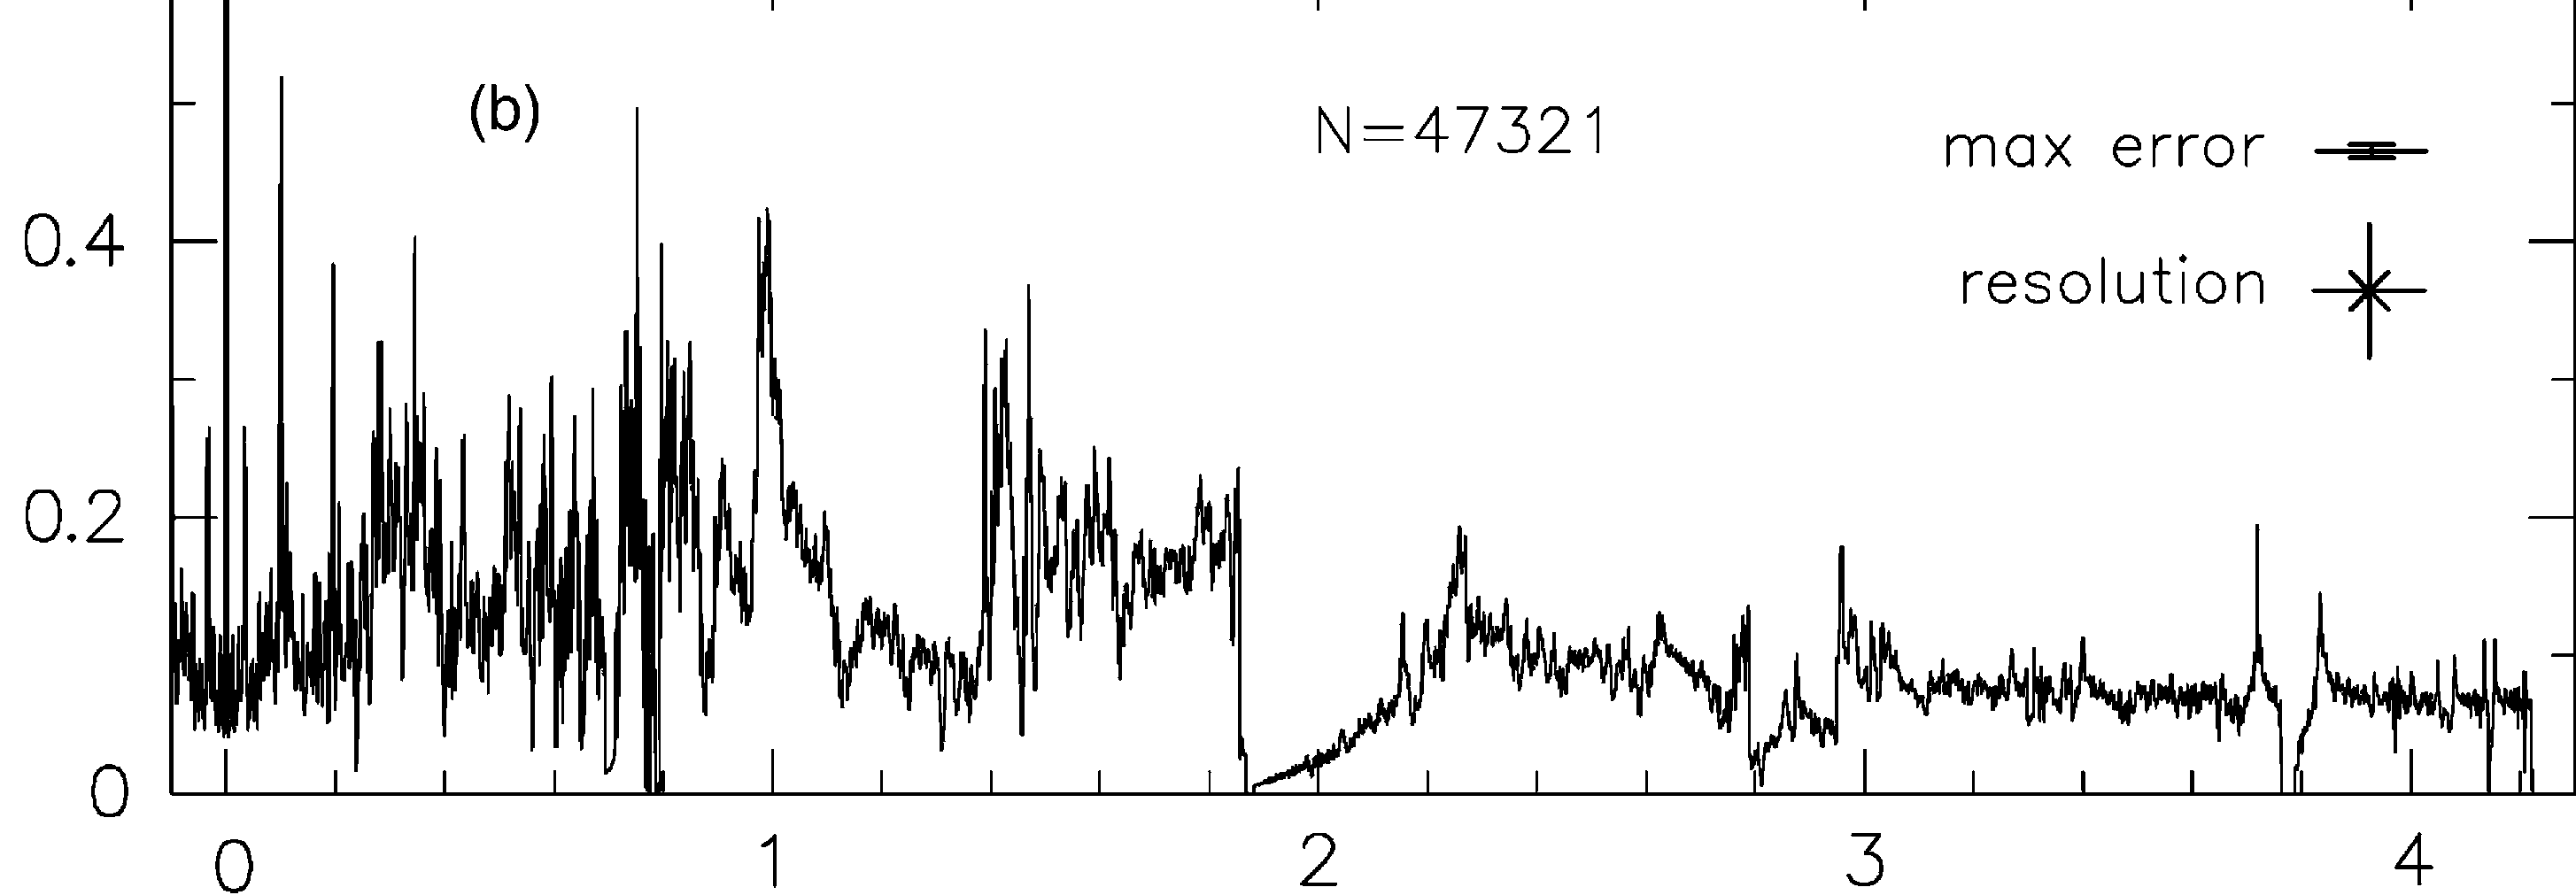
\includegraphics[scale=.1]{img/idos_AB_small.png}

}
\begin{itemize}
	\item Spectrum: no apparent fractal structure
	\item States are critical (numerical result, eg [Rieth, Schreiber 1998])
\end{itemize}
$\rightarrow$ can we introduce a field of arrows to describe some of these critical wavefunctions?
\end{frame}

\begin{frame}{A natural field of arrows}

In superspace, arrows go from the center to the border of the slice:

{\centering
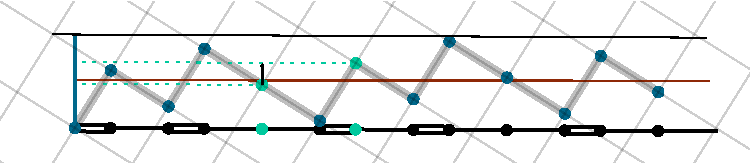
\includegraphics[scale=.8]{img/cut_and_project_arrows.pdf}

}

\begin{columns}
\<{7cm}
\begin{itemize}
	\item Define arrows in the same way for 2D tilings (they coincide with the \emph{matching rules})
	\item Consider again the height: $h(m) = \sum A$
\end{itemize}
	Can we describe states with this arrow field? $\psi_m = \rho^{h(m)}$ (with $\rho$ a constant)
\>
\<{7cm}
{\centering
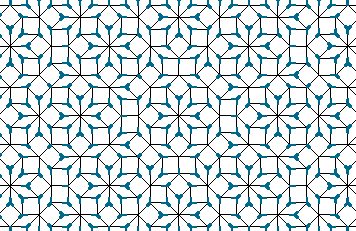
\includegraphics[scale=1.]{img/arrowed_tiling_excerpt.pdf}

}
\>
\end{columns}

\end{frame}

\begin{frame}{The groundstate wavefunction}
Can we find an ``arrowed state'' $\psi_m = \rho^{h(m)}$ ? (with $\rho$ a constant)
\begin{itemize}
\item Idea [Sutherland 1986]: tune the potential
\[
	E \psi_m = V_m \psi_m + t \sum_{n ~\text{NN}~m} \psi_n \Longleftrightarrow V_m = E - t\sum_n \rho^{A_{m,n}}
\]
Obtain a groundstate which is an arrowed state.

Not very physical! Generically, potential is not finely tuned.

\item Guess [Kalugin, Katz 2014]: state still arrowed, but with a local modulation:
\[
	\psi_m = C_{m} \rho^{h(m)}
\]
where $C_m$ is local:
\[
	C_m \simeq C_n \text{~ if the tiling looks the same around $m$ and $n$}
\]
\end{itemize}
\end{frame}

\begin{frame}{Robustness of the structure}

\begin{columns}
\<{8cm}
\includegraphics[scale=.5]{img/gs.png}
\>
\<{6cm}
\begin{itemize}
\item The groundstate is \textbf{very robust}: 

For any model of the form
\[
	E \psi_m = V_m \psi_m + t\sum_{n} \psi_n
\]
the groundstate is an ``arrowed state''
\[
  \psi_m = C_m \rho^{h(m)}
\]
\item Same arguments as in 1D: the state has power law decay, and is critical.
\end{itemize}
$\rightarrow$ what can we do now?
\>
\end{columns}
\end{frame}

\begin{frame}{Scaling of the groundstate}

\begin{columns}
\<{7cm}
\begin{itemize}
	\item Participation ratio over a region $\mathcal{R}$:
	\[
		\text{PR}(\psi, \mathcal{R}) = \frac{\left( \sum_{m \in \mathcal{R}}|\psi_m|^2 \right)^2}{\left( \sum_{m\in \mathcal{R}} |\psi_m|^4 \right)^4}
	\]
	\item Scaling with the region volume $\text{Vol}(\mathcal{R})$:
	\[
		\text{PR}(\psi, \mathcal{R}) \sim \text{Vol}(\mathcal{R})^{D(\psi)}
	\]
	\begin{itemize}
		\item $D(\psi) = 0 \implies \psi$ localized
		\item $D(\psi) = 1 \implies \psi$ extended
		\item $0 < D(\psi) < 1 \implies \psi$ critical
 	\end{itemize}
\end{itemize}
\>

\<{7cm}
We can compute the scaling analytically for the groundstate:
\[
\boxed{
D(\psi) = \log\left( \frac{\omega(\rho^2)^2}{\omega(\rho^4)}\right)/\log \omega(1)
}
\]
with (for Ammann-Beenker)
\begin{align*}
\omega(z) &= \frac{a(z)+\sqrt{a(z)^2 - z^2}}{z} \\
a(z) &= 4 z^2 + 9 z + 4
\end{align*}
Scaling only depends on the arrow distribution, only on the \textbf{geometry} of the tiling.
\>
\end{columns}
\end{frame}

\section{Conclusion and perspectives}
\subsection{Dummy}
\begin{frame}{Conclusion}
\begin{itemize}
	\item Examples of generic \textbf{critical} eigenstates.
	\begin{itemize}
		\item 1D (Fibonacci): the $E=0$ state
		\item 2D (Penrose and Ammann-Beenker): the groundstate.
	\end{itemize}
	\item Geometry $\rightarrow$ quasiperiodic \textbf{arrow function} $\rightarrow$ structure of the state.
	\item In 2D, structure \textbf{robust to changes in the model} (varying potential, hopping)
	\item Using this description, we can easily compute physical observables.
\end{itemize}
Perspectives:
\begin{itemize}
	\item For Penrose and Ammann-Beenker, the arrow field is not enough to describe excited states. Extra ingredients?
	\item Other 2D quasicrystals: generalized Penrose, dodecagonal \dots
\end{itemize}
\end{frame}

%%%%%%%%%%%% Extra slides %%%%%%%%%%%%%
\begin{frame}{Cut and project chains are special!}
Consider the chain constructed by the substitution
\begin{align*}
	A & \to ABBB \\
	B & \to A
\end{align*}
\begin{columns}
\<{6cm}
\begin{itemize}
	\item This substitution cannot be built by cut and project (because it is non-Pisot).
	\item Height resembles a random walk, and typical height $\sim \sqrt{L}$
	\item As a result, the wavefunction is localized! 
\end{itemize}
\>
\<{6cm}
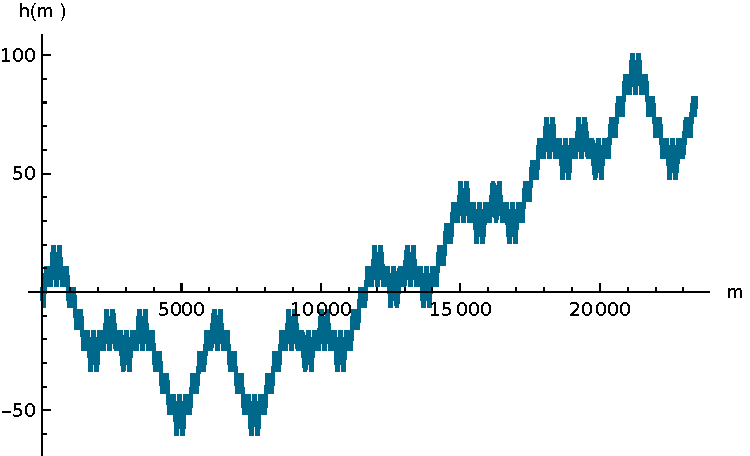
\includegraphics[scale=.5]{img/heightsB3.pdf}
\>
\end{columns}
$\rightarrow$ criticality is sensitive to the \textbf{complexity} of the tiling
\end{frame}

\begin{frame}{Theory/numerics on the 2D groundstate}
\begin{columns}
\<{7cm}
\centering
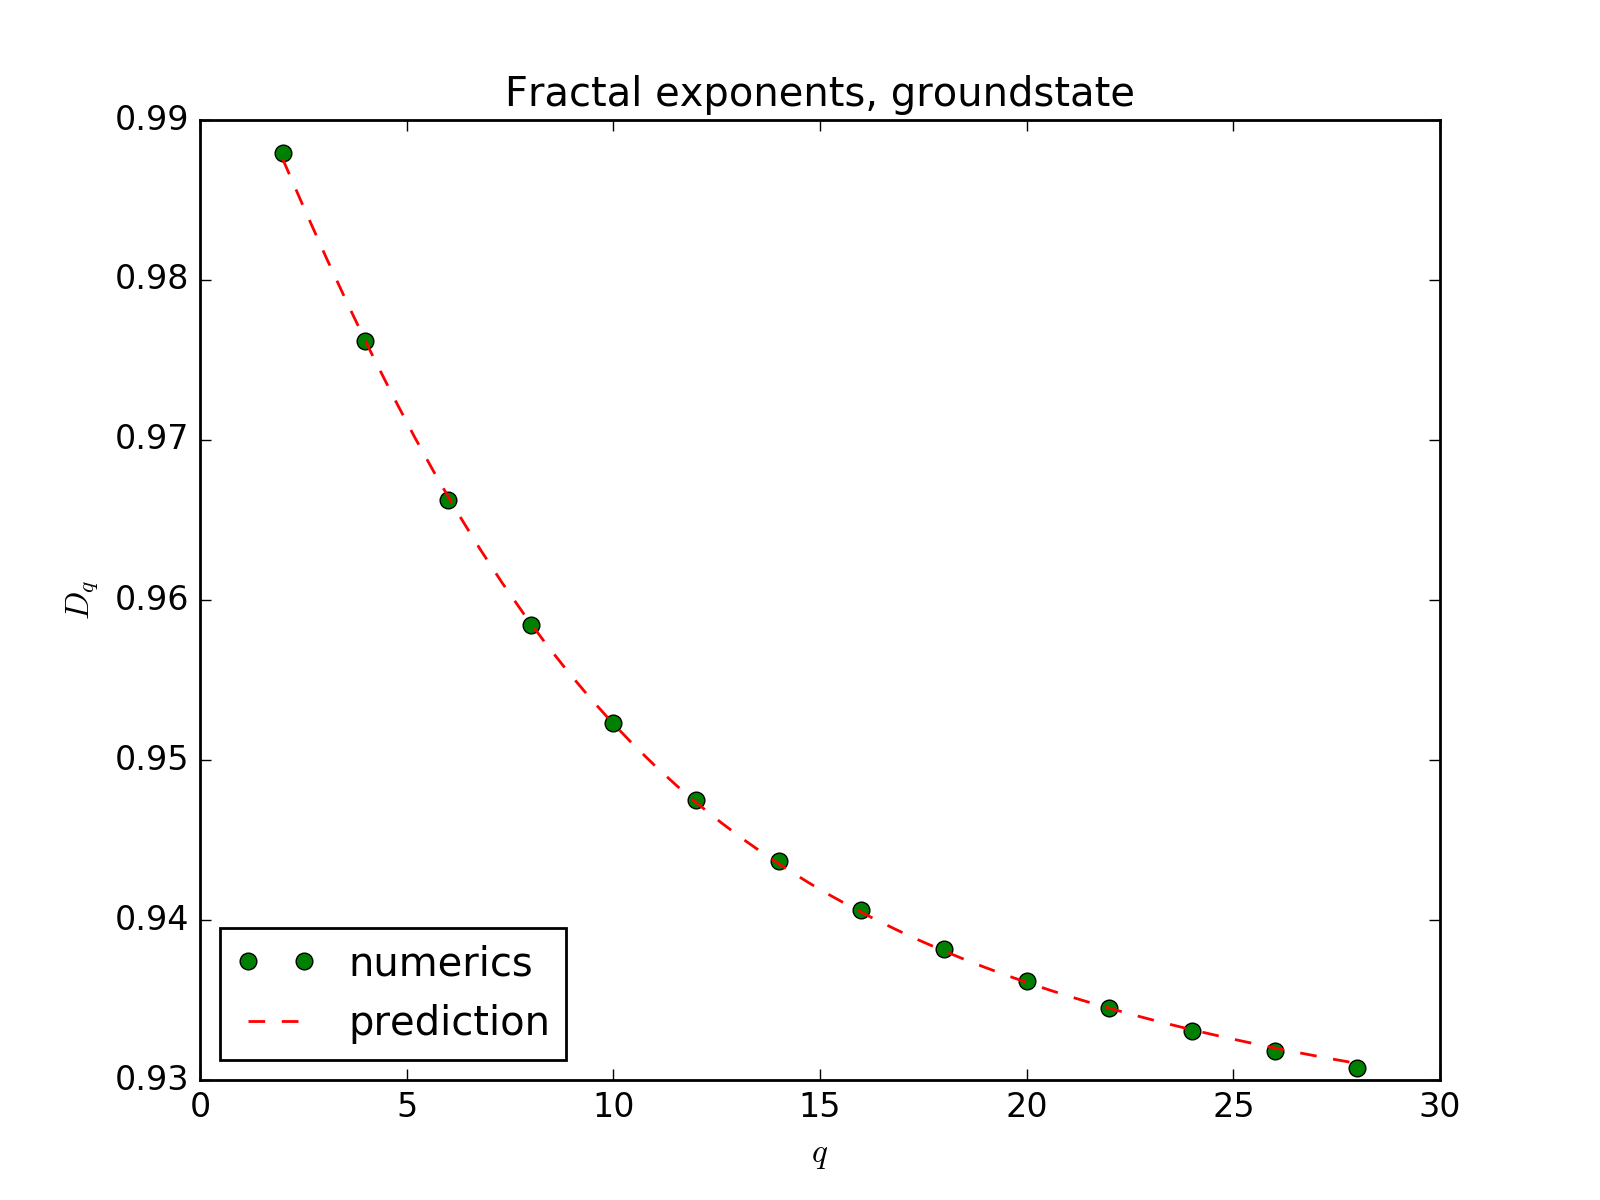
\includegraphics[scale=.4]{img/fractal_exponents_groundstate.png}
\>
\<{7cm}
\[
	t \sum_{n ~\text{NN}~m} \psi_n + (t-1)z_m \psi_m = E \psi_m
\]
\centering
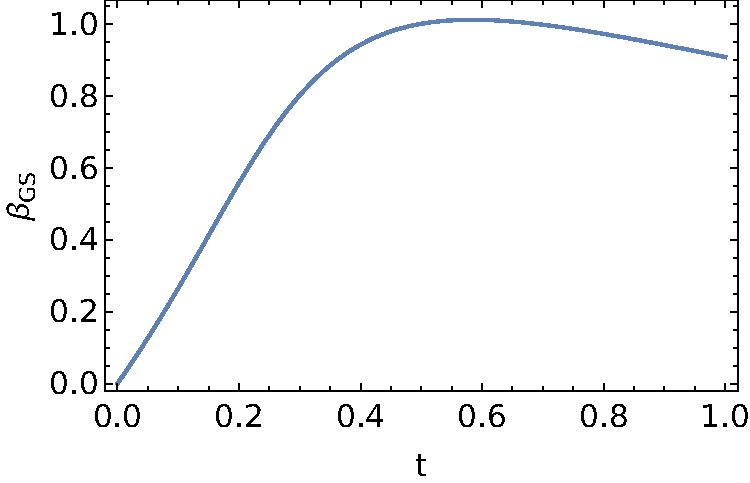
\includegraphics[scale=.6]{img/beta_t.pdf}
\[
	\psi_m = C_m \beta^{h(m)}
\]
\>
\end{columns}
\end{frame}

\begin{frame}{Computation of a local observable}
Compute the local observable $\hat{O}$, in the $\psi$ state: $\braket{\psi | \hat{O} | \psi}$

Assumptions:
\begin{itemize}
	\item The observable only depends on the local configuration of the atoms.
	\item The state is described by an arrow field and a local variation: $\psi_m = C_m \rho^{h(m)}$
\end{itemize}
\[
	\braket{\psi | \hat{O} | \psi} = \sum_{m,n} \psi_m^* \hat{O}_{m,n} \psi_n
\]
\[
\boxed{\braket{\psi | \hat{O} | \psi} = \sum_{\mu, \nu}C_{\mu}^* \hat{O}_{\mu,\nu} C_{\nu} \sum_{h,h'} f(\mu, h; \nu, h') \rho^{h+h'}}
\]
\end{frame}

\end{document}